\documentclass[a4paper]{article}

%Appearence ----------------------
\usepackage{titling}
\newcommand{\subtitle}[1]{%
  \posttitle{%
    \par\end{center}
    \begin{center}\large#1\end{center}
    \vskip0.5em}%
}
\usepackage{indentfirst}
\usepackage[font={small}]{caption}
\usepackage{geometry}
\geometry{
  margin=2.54cm
}

%Portuguese packages ----------
\usepackage[utf8]{inputenc}
\usepackage[portuguese]{babel}

%Add-ons -----------------------------
\usepackage{booktabs}
\usepackage{graphicx}
\usepackage{amsmath}	
\usepackage{amsfonts}	
\usepackage{tabu}

\title{Relatório de Electromagnetismo I}
\subtitle{Estudo da histerese de um material ferromagnético}
\author{André Duarte, Marcos Gouveia e Sagar Pratapsi}	
\date{3 de Dezembro de 2013}

\begin{document}

\maketitle

\section{Objectivos}
Quando um material ferromagnético é colocado numa zona onde existe um campo $\mathbf{H}$, cria um campo de magnetização, $\mathbf{M}$, sendo que o campo magnético resultante na região é dado por \begin{equation}\label{campos} \mathbf{B}=\mu_0\left( \mathbf{H}+\mathbf{M}\right).\end{equation} Esta magnetização, no entanto, não é apenas uma função do campo externo aplicado, mas também da magnetização pré-existente no material. Existe um efeito de memória a que se chama histerese. 

O objectivo deste trabalho foi obter e analisar a histerese de um material (chave de parafusos) medindo vários valores de $\mathbf{B}$ junto ao mesmo em função do campo $\mathbf{H}$, aplicado por um solenóide. Na Secção 2 explicamos o procedimento utilizado e a razão pela qual o campo $\mathbf{B}$ é uma medida aceitável da magnetização.
\section{Métodos}
Para estudar a curva de histerese, utilizamos uma chave de parafusos, que colocámos no centro de uma bobina. Na bobina fez-se passar uma corrente eléctrica, alimentada por uma fonte de alimentação que permitia variar a intensidade da corrente - medida por um multímetro colocado em série. Assim foi possível criar no centro da bobina um campo magnético, dado aproximadamente por $\mathbf{H}=nI$, sendo $n=1500$ o número de espiras e $I$ a intensidade da corrente. Depois de colocada a chave de parafusos no interior do solenóide, variou-se a intensidade da corrente aplicada e mediu-se o campo $\mathbf{B}$ resultante. Apesar de existirem simultaneamente os campos $\mathbf{H}$ e $\mathbf{M}$ quando a chave se encontra no solenóide, este último tem uma ordem de grandeza consideravelmente superior ao primeiro, pelo que a Equação \ref{campos} pode ser aproximada por $\mathbf{B} \approx \mu_0 \mathbf{M}$. Assim, $\mathbf{B}$ é uma boa estimativa do campo de magnetização.

\subsection{Determinação dos campos $ \mathbf{H}$ e $ \mathbf{B}$}
Para medir os campos magnéticos, usou-se um sensor de Hall (ref.\ SS490A1) que devolve uma diferença de potencial $V$ em função da magnitude do campo detectado, $B$. A curva de calibração que relaciona estes valores é \begin{equation}\label{calibracao}B=320V-800,\end{equation}
com $B$ em Gauss e $V$ em Volt.

O sensor apenas mede o campo \textbf{B} total existente numa região. No entanto, para o nosso objectivo, é necessário determinar o campo \textbf{H} existente independentemente do material ferromagnético. Para isso, dividimos a experência em duas partes:
\begin{enumerate}
\item Medir o campo magnético $B$ sem a chave de parafusos no solenóide, em função da intensidade da corrente $I$ utilizada.  Determinar a expressão para a curva $H(I)$, sabendo que neste caso $H=B/\mu_0$.
\item Medir o campo magnético $B$ com a chave de parafusos no solenóide, em função da corrente $I$ utilizada.
\end{enumerate}

Com base na curva de calibração determinada na primeira parte e nos valores de $I$ obtidos na segunda, podemos determinar o campo $H$ existente quando o ferromagnete se encontra presente. O campo $B$ da segunda parte da experiência, como já vimos, dá-nos a magnetização do material.

Com os resultados obtidos, realizámos um gráfico de $B(H)$ na presença do ferromagnete, para observar a curva de histerese.

\section{Resultados}
\begin{figure*}[htbp]
\centering
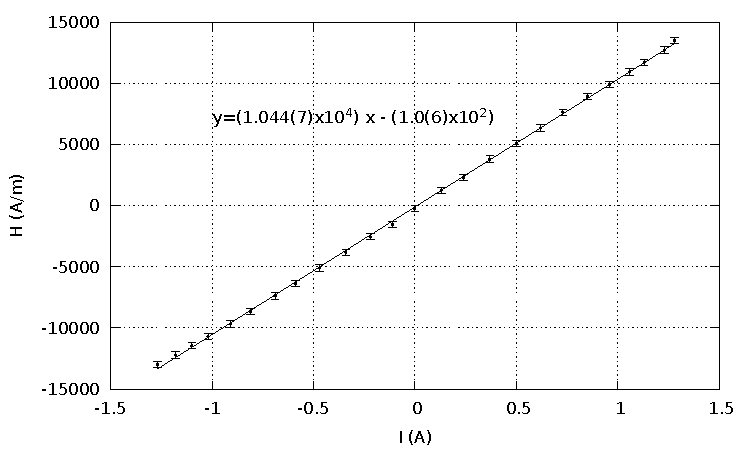
\includegraphics[width=0.7\textwidth]{./Imagens/grafico1.pdf}
\caption{Curva de calibração de $H$ em função de $I$.}
\end{figure*}

\begin{figure*}[htbp]
\centering
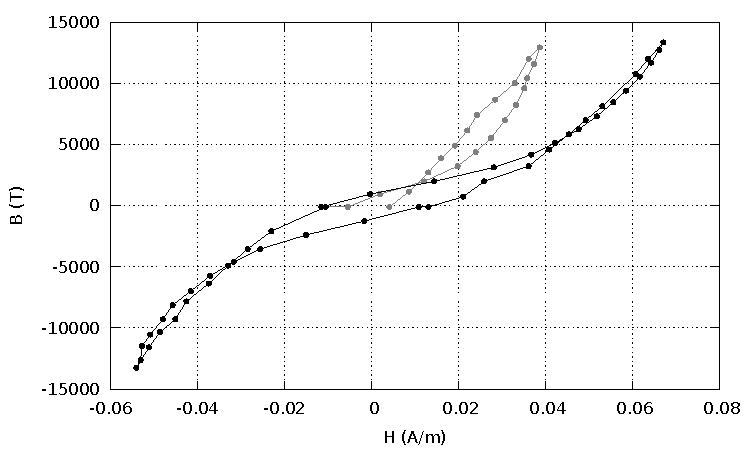
\includegraphics[width=0.7\textwidth]{./Imagens/grafico2.pdf}
\caption{Curva de histerese: campo medido $B$ em função de $H(I)$, determinado pela recta de calibração.}
\end{figure*}

\section{Análise e discussão dos dados}
\section{Anexos}
\subsection{Cálculo dos erros associados às medidas}
Na secção 3, as grandezas obtidas foram medidas directamente, pelo que os erros foram estimados tendo em conta o método de medição usado. No entanto, na secção 4, as grandezas foram calculadas a partir das obtidas directamente, pelo que há propagações de erros envolvidas. Esses erros foram calculados pela fórmula de propagação de erros: \begin{equation} \delta f(x_1,x_2,\ldots,x_n)=\sqrt{\sum_{i=1}^{n}\left( \frac{\partial f}{\partial x_i}\delta x_i \right)^2}\end{equation}.

Aqui, $f$ é uma grandeza calculada a partir das grandezas $x_1,x_2,\ldots,x_n$, e $\delta x_i$ são os erros associados às mesmas. Na Tabela 4 apresentamos as equações das grandezas calculadas bem como os respetivos erros.
\renewcommand{\arraystretch}{2.5}
\begin{table}[htbp]
\begin{center}
\caption{Resumo das equações utilizadas para efectuar o cálculo de grandezas relevantes e o respectivo erro, calculado pela fórmula de propagação de erros - equação (4).}
\begin{tabular}{lll}
\textbf{Grandeza} & $f(x_1,x_2,\ldots,x_n)$ & $\delta f(x_1,x_2,\ldots,x_n)$ \\ \hline
\textbf{Área}&$\displaystyle A=\pi\left(\frac{d}{2}\right)^2 $ & $\displaystyle \delta A= \frac{\pi d}{2}\delta d $ \\
\textbf{Área média} &$\displaystyle A_g=\frac{A_i+A_f}{2}$ & $ \displaystyle\delta A_g=\frac{1}{2}\sqrt{\delta A_i^2+\delta A_f^2}$ \\
\textbf{Taxa de fusão} &$\displaystyle R=R_a=\frac{m_f-m_i}{\Delta t}$&$ \displaystyle\delta R=\delta R_a= \sqrt{\left( \frac{\delta m_i}{\Delta t}\right)^2+\left( \frac{m_f}{\Delta t}\right)^2+\left( \frac{m_f-m_i}{\Delta t^2}\delta(\Delta t)\right)^2}$ \\
\textbf{Taxa de fusão efectiva}&$\displaystyle R_0=R-R_a$ & $ \displaystyle \delta R_0= \sqrt{\delta R^2+\delta R_a^2}$ \\
\textbf{Condutividade}&$\displaystyle k=\frac{R_0 L_g h}{A_g \Delta T} $& $ \displaystyle \delta k= k\sqrt{\left(\frac{\delta R_0}{R_0}\right)^2+\left(\frac{\delta h}{h}\right)^2+\left(\frac{\delta A_g}{A_g}\right)^2}$ \\ [2ex] \hline
\end{tabular}
\end{center}
\end{table}

\end{document}